\section{Termpot}\label{sec:termpot}

O Termpot (ver Figura \ref{fig:termpot}) é um ambiente para improvisação de luteria composicional \cite{iazzetta_musica_2009,soares_luteria_2015}, mais especificamente, um ambiente \emph{web} de \emph{livecoding}. Adapta o ambiente \emph{Wavepot} (apresentado na nota-de-rodapé 2 da Seção \ref{sec:introducao}) para um emulador de terminal, controlado pela linguagem \emph{coffeescript}\cite{burnham2011coffeescript}\footnote{\url{http://coffeescript.org/}, acessado em \today.}. O ambiente possibilita a improvisação de códigos com a extensão média de uma linha (ver Código \ref{code:resultado1}). 

\begin{figure}[!h]
\centering
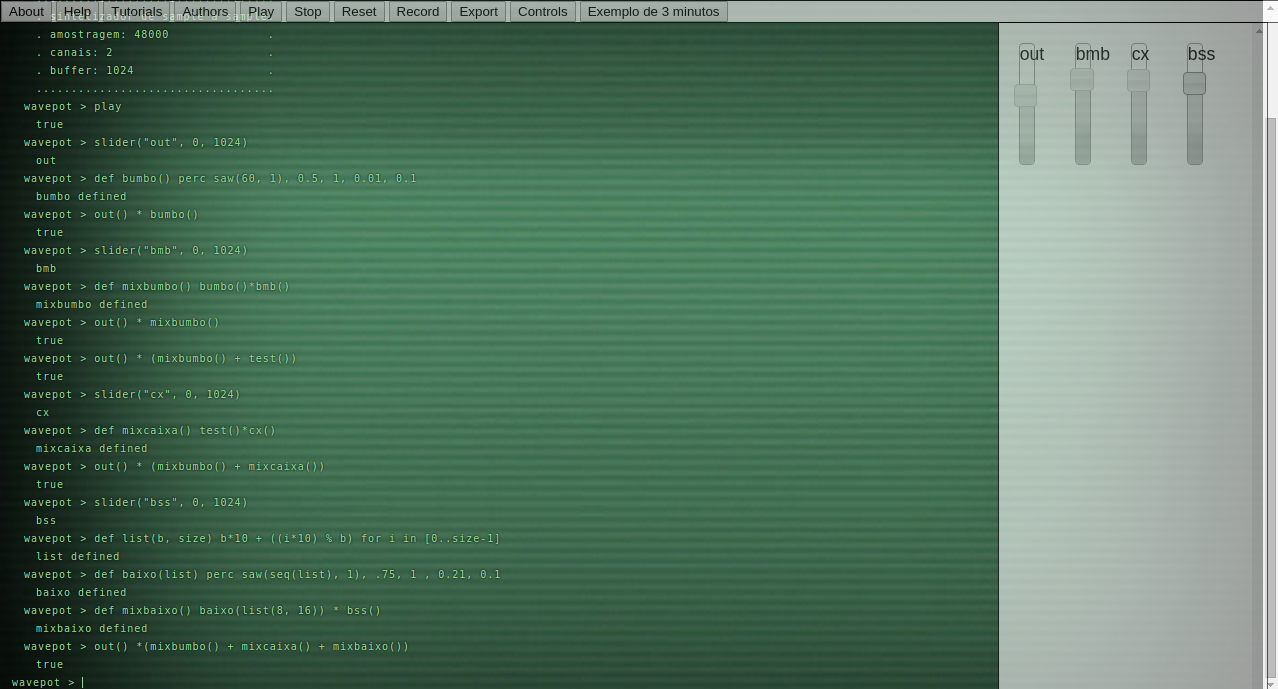
\includegraphics[scale=0.35]{termpot.png}
\caption{Aplicativo \emph{Termpot}. \textbf{Fonte}: autores.}
\label{fig:termpot}
\end{figure}

\begin{listing}
\begin{minted}[linenos,frame=lines,framesep=2mm,fontsize=\scriptsize]{javascript}
.........................................
. Virtual machine started at             .
. Thu Sep 03 2015 13:32:15 GMT-0300 (BRT).
. type help for instructions             .
..........................................
$\$$ |
$\$$ wavepot 1024
..................................
. sintetizador de sample a sample. 
. amostragem: 44100              .
. canais: 2                      .
. buffer: 1024                   .
..................................
wavepot > play
wavepot > 0.71 * sin 440, sin(330, sin(220, 0.5)
true
\end{minted}
\caption{Console do \emph{termpot} aguardando dados de entrada do improvisador; o improvisador inicia o ambiente wavepot com um buffer de 1024 pontos flutuantes; o improvisador inicia o processamento de áudio; o improvisador define o processamento de áudio de uma cascata de Modulção de amplitude.}
\label{code:resultado1}
\end{listing}

Em tese, é possível criar sonoridades semelhantes ao \emph{Wavepot}. Porém, dado o curto tempo de desenvolvimento, pré-definimos apenas ruído (branco), senóide, dente-de-serra, triangular, pulso, envelope e sequenciamento.

É possível prototipar rapidamente novas funções para encapsular novas funcionalidade sonoras ao ambiente.

\begin{listing}
\begin{minted}[linenos,frame=lines,framesep=2mm,fontsize=\scriptsize]{javascript}
wavepot > def tresAM(f, f1, f2, a) a * sin f, sin(f1, sin(f2, 0.5)
true
wavepot > inspect tresAM
var tresAM;

tresAM = function(f, f1, f2, a) {
  return a * sin(f, sin(f1, sin(f2, 0.5)))
};
wavepot > tresAM 440, 330, 220, 0.71 
\end{minted}
\label{code:resultado2}
\end{listing}

Além da atividade de síntese, elaboramos uma maneira para a criar e utilizar GUIs de controle (\emph{sliders}), como uma mesa de som (ver Código \ref{code:resultado3}

\begin{listing}
\begin{minted}[linenos,frame=lines,framesep=2mm,fontsize=\scriptsize]{javascript}
wavepot > slider("left", 0, 1024)
true
wavepot > slider("right", 0, 1024)
true
wavepot > stereo sin(440,0.5)*left(), sin(330, 0.5)*right()
true
\end{minted}
\caption{Exemplo de código do Wavepot}
\label{code:resultado3}
\end{listing}


Uma característica singular do \emph{Wavepot} original, é a possibilidade de separação da programação-partitura em dois arquivos, muito semelhante ao método \emph{Instrumento-Orquestra} descrito por Max Mathews e utilizado no CSound \cite{mathews_digital_1963, di_nunzio_genesi_2010}.
Isso é possível adicionando um marcador $@module$ aos comentários iniciais de um código.
Desta forma, serão reconhecidos dois arquvivos durante a performance de improvisação: $index.js$ e $test.js$.
O primeiro permite elaborar os instrumentos, enquanto o segundo realiza o DSP (teste).

Já no Termpot, buscamos utilizar outro método de codificação focado em uma abordagem mais performática.


Arriscamos a comentar uma inspiração no GROOVE de \cite{mathews_groove_1970,nunzio_groove_2010}, quando este propõe a criação de novas funções em tempo de execução. Ao mesmo tempo em que utilizamos a biblioteca \emph{Ptty.js} dando ao \emph{Termpot} as características de um emulador de terminal no que tange a utilização de comandos em tempo de execução, como em um terminal, integrado com controles manuais.
Por esta razão, acreditamos que esta ferramenta é inspirada no conceito de compor, memorizar, editar e controlar funções do tempo, algoritmicamente e manualmente~\cite{mathews_groove_1970}.


%\subsection*{Metodologia de desenvolvimento}

%Para a implementação, três tarefas foram necessárias: \begin{description}
%\item[1) Customizar um emulador terminal]
%\item Utilizamos a biblioteca \emph{Ptty.js} é uma biblioteca documentada e pode ser facilmente implementada seguindo instruções de seu arquivo \emph{README}. É baseada em jQuery e permitiu uma rápida prototipação.
%\item[2) Implementar um ambiente de síntese sonora integrado ao emulador]
%\item Uma das facilidades do \emph{Ptty} é definir ambientes; elaboramos um ambiente que controla a \emph{Web Audio API} nos moldes descritos na Seção 2.
%\item[3) Comandos diversos]
%\item Ajuda, inspeção de funções, definição de novas funções, tocar, parar, pausar, gravar e download e criação de controles gráficos. Para gravação, utilizamos o \emph{recorderWorker.js}\footnote{\url{https://github.com/mattdiamond/Recorderjs/blob/master/recorderWorker.js}.} de Matt Diamond.
%\end{description}
